\documentclass[12pt]{article}
\usepackage{url,setspace,amsmath}
\usepackage{graphicx}
\setlength{\oddsidemargin}{-8mm}
\setlength{\evensidemargin}{0mm}
\setlength{\textwidth}{175mm}
\setlength{\topmargin}{-5mm}
\setlength{\textheight}{240mm}
\setlength{\headheight}{0cm}
\setstretch{1}

\begin{document}
\title{\vspace{-2cm}Documentation for chainBD: minimalist code for Brownian dynamics of a semiflexible chain}
\author{E.~F.~Koslover}
\date{Last updated \today}
\maketitle

The code in this package will run a simple Brownian dynamics simulation of a semiflexible chain. 

%\tableofcontents
%\newpage

\section{Compilation Instructions}
To compile and run the program, you will need the following:
\begin{itemize}
\item a compiler capable of handling Fortran90.
The code has been tested with the gfortran and compiler. The default compiler is gfortran.
\item BLAS and LAPACK libraries installed in a place where the compiler knows to look for them
\item Optionally: Matlab to visualize output data
\end{itemize}

The code has been tested on Ubuntu Linux. 

To compile with gfortran, go into the \path=source= directory. Type \verb=make=.
To compile with any other compiler that can handle Fortran90, type
\begin{verbatim}
make FC=compiler
\end{verbatim}
substituting in the command you usually use to call the compiler. 

If the compilation works properly, the executable \path=chainBD.exe= will appear in the main directory.

\section{Usage Instructions}
To run the program in the main directory, type:
\begin{verbatim}
./chainBD.exe suffix > outputfile.out
\end{verbatim}

Here, \verb=suffix= can be any string up to 100 characters in length. 
The program reads in all input information from a file named
\path=param.suffix= where, again, \verb=suffix= is the command-line
argument. If no argument is supplied, it will look for a file named
\path=param=. If the desired parameter file does not exist, the
program will exit with an error. You can supply multiple suffixes to read in multiple parameter files.

The parameters in the input file are given in the format "{\em KEYWORD} value" where the possible keywords and values are described
in Section \ref{sec:keywords}. Each keyword goes on a separate
line. Any line that starts with "\#" is treated as a comment and
ignored. Any blank line is also ignored. The keywords in the parameter
file are not case sensitive. For the most part, the order in which the
keywords are given does not matter. All parameters have default
values, so you need only specify keywords and values when you want to
change something from the default.


\section{Example for a Quick Start}
\subsection{Example 1}
An example parameter file (\verb=param.example1=) is provided. This will run a Brownian dynamics simulation for a short, approximately Gaussian chain (low bending modulus). Run the example with 
\begin{verbatim}
./chainBD.exe example1
\end{verbatim}

Use the script \verb=checkexample.m= to visualize the resulting MSD of a bead at the end of the chain. It should look something like this:

\centerline{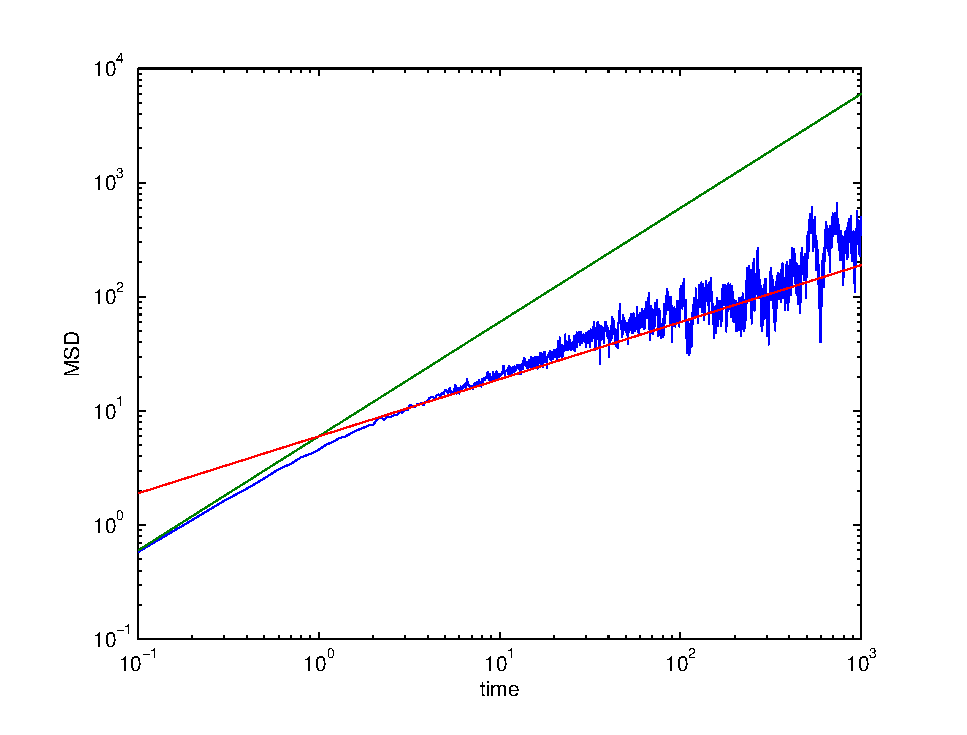
\includegraphics[width=0.7\textwidth]{example_MSD.eps}}

\subsection{Example 2}
Example 2 runs Brownian dynamics on a chain with one end fixed and the other end pulled continuously in the z direction. Use the script \verb=example2.m= to visualize the configuration of the chain over time.

% ---------------------------------------------------------

\section{Keyword Index}
\label{sec:keywords}
The code will attempt to read parameters out of a file named \path=param.suffix= where ``suffix'' is the command line argument. If no command line arguments are supplied, it will look for a file named \path=param=. If multiple arguments are supplied, it will read multiple parameter files in sequence.

The parameter file should have one keyword per line and must end with a blank line. All blank lines and all lines beginning with \# are ignored. For the most part, the order of the lines and the capitalization of the keywords does not matter. All keywords except {\em ACTION} are optional. The default values for each parameter are listed below. If a keyword is supplied, then values may or may not be needed as well. Again, the required and optional value types are listed below. 

Keywords and multiple values are separated by spaces. 

When reading the parameter file, lines longer than 500 characters will be truncated. To continue onto the next line, add ``+++'' at the end of the line to be continued.
No individual keyword or  value should be longer than 100 characters.

Floating point numbers can be formated as $1.0$, $1.1D0$, $10e-1$, $-1.0E+01$, etc., where the exponential notation specifier must be D or E (case insensitive). Integer numbers can also be specified in exponential notation without decimal points (eg: 1000 or 1E3). Logical values can be specified as T, F, TRUE, FALSE, 1, or 0 (with 1 corresponding to true and 0 to false).

The length units used for the defaults are in nm and the energy units are in kT. 

\begin{itemize}
%
\item {\it ACTION}
  \begin{itemize}
    \item  value: 1 string of at most 20 characters; no default
    \item This keyword sets the overall calculation performed by the program (see Sec.\ref{sec:tasks})
    \item Possible values are: BROWNDYN
  \end{itemize}
%
\item {\it BDPRINTEVERY}
  \begin{itemize}
    \item  value: 1 integer; default 1
    \item How often to print output to screen and to the output file (given by {\em OUTFILE})
  \end{itemize}
%
\item {\it BDSTEPS}
    \begin{itemize}
      \item  value: 1 integer; default 1000
      \item Number of Brownian dynamics steps to run
    \end{itemize}
%
\item {\it DELT}
    \begin{itemize}
      \item  value: 1 float; default 1D-4
      \item Time-step for the Brownian dynamics
    \end{itemize}
%
\item {\it DELT}
    \begin{itemize}
      \item  value: 1 float; default 1D-4
      \item Time-step for the Brownian dynamics
    \end{itemize}
%    
\item {\it ESTR}
    \begin{itemize}
      \item  value: 1 float; default 1000
      \item Stretch modulus for individual segments
    \end{itemize}
%    
\item {\it EXTFORCE}
    \begin{itemize}
      \item  value: 1 integer, 3 floats; default: none
      \item Apply an external force to a specific bead of the chain. 
      \item Lists the bead index followed by x, y, z components of the force
      \item Multiple lines (up to 1000) can be used to apply forces on multiple beads
    \end{itemize}
%    
\item {\it FIXBEADS}
    \begin{itemize}
      \item  value: up to 1000 integer values
      \item Fix the listed beads (prevent them from moving).
    \end{itemize}
%    
\item {\it FRICT}
    \begin{itemize}
      \item  value: 1 float; default: 1D0
      \item Frictional coefficient for Brownian dynamics
    \end{itemize}
%    
\item {\it KT}
    \begin{itemize}
      \item  value: 1 float; default: 1D0
      \item Temperature ($k_b T$) for Brownian dynamics
    \end{itemize}
%    
\item {\it LP}
    \begin{itemize}
      \item  value: 1 float; default: 1D0
      \item Persistence length of the semiflexible chain
    \end{itemize}    
%    
\item {\it LS}
    \begin{itemize}
      \item  value: 1 float; default: 1D0
      \item Segment length for the chain
    \end{itemize}   
%    
\item {\it LS}
    \begin{itemize}
      \item  value: 1 float; default: 1D0
      \item Segment length for the chain
      \end{itemize}
 %    
 \item {\it NOBROWN}
     \begin{itemize}
       \item  value: none
       \item Turn off random Brownian forces (equivalent to zero temperature dynamics)
     \end{itemize}   
%    
\item {\it OUTFILE}
    \begin{itemize}
      \item  value: 1 string, up to 100 characters; default: *.out
      \item Output file for energy and coordinates of last bead.
      \item Any * in the file name will be replaced by the command-line argument (suffix)  
      \end{itemize}
%    
\item {\it RNGSEED}
  \begin{itemize}
    \item 1 integer; default: 0
    \item seed for random number generator
    \item value of 0 will seed with system time in milliseconds
    \item value of -1 will use the last 5 characters in the suffix
    \item value of -2 will use the last 4 charactes in the suffix and the millisecond time
    \item other positive value: the seed is used directly for repeatable simulations (should be positive)
  \end{itemize}
%
\item {\it SNAPSHOTS}
  \begin{itemize}
    \item 1 optional integer, 1 optional string, 1 optional logical; defaults: 1, *.snap.out, false 
    \item Dump snapshots over the course of the calculation
    \item integer: how often to dump snapshots; string: snapshot file (* is replaced with suffix); logical: append rather than rewriting the snapshot file
   \end{itemize}
%
\item {\it SNAPSHOTFILE}
    \begin{itemize}
      \item  value: 1 string; default: *.snap.out
      \item File for dumping out snapshots. Can also be specified within SNAPSHOTS keyword.   
    \end{itemize} 
%
\item {\it STARTEQUIL}
    \begin{itemize}
      \item  value: 1 optional logical; default: false if keyword not supplied, true if keyword supplied without arguments
      \item If true, chain is started from equilibrium configuration
      \item If false, chain is started from straight configuration
    \end{itemize} 
%
\item {\it VERBOSE}
        \begin{itemize}
          \item  value: 1 logical; default: false 
          \item Print extra output. Not currently implemented
        \end{itemize} 
% --------------------------

\end{itemize}

\bibliographystyle{aip} 
\bibliography{fiberModel}

\end{document}
